% D.22 ⊙O 直径 AB，C、D 在圆上，∠BAC=35°，∠ABD=50°
\documentclass[tikz,border=4pt]{standalone}
\usepackage{ctex}
\usepackage{amsmath}
\usetikzlibrary{calc}
\begin{document}
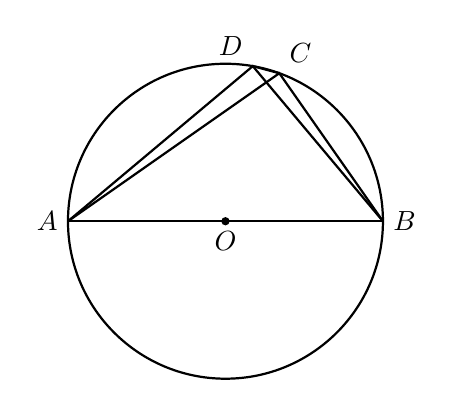
\begin{tikzpicture}[scale=1.0, thick]
  \coordinate (O) at (0, 0);
  \draw (O) circle (2);
  \coordinate (A) at (-2, 0);
  \coordinate (B) at ( 2, 0);
  % C 上半圆：∠BAC=35° → C = A + t·(cos35°, sin35°)，且在圆上
  % 用圆周角：∠AOC = 2·∠ABC，但更简单：取 C 使 ∠BAC=35°
  % 方向角 35° 从 A 出发，与圆相交：
  \coordinate (C) at ({-2 + 4*cos(35)*cos(35)*2}, 0); % placeholder
  % 用更简单方法：直接根据 ∠ACB=90°（C 在以 AB 为直径的圆上），C 满足 ∠BAC=35° → 在 AB 上方
  % C = (cos(2·35°-180°)*r + 0, sin(...)*r) 实际：C 角参数 θ 使 AC 与 AB 夹 35°
  % 圆心角 ∠AOC = 180°-2·35°=110°，C = O + r·(cos(180-110), sin(180-110)) = (cos70°, sin70°)·2
  \coordinate (C) at ({2*cos(70)}, {2*sin(70)});
  % ∠ABD=50° → 圆心角 ∠AOD（D 一侧）= 180°-2·50°=80°，但 D 与 C 应不同位置
  % 取 D 在下半圆：∠AOD（从正 x 反向量起）使 BD 与 BA 成 50°
  % 圆心角 ∠BOD = 2·∠BAD（如 D 在异侧），简化：让 D 在上半圆 BD 方向 (cos(180-50), sin(180-50))=(-cos50, sin50)
  \coordinate (D) at ({2*cos(180-2*50)}, {2*sin(180-2*50)});

  \draw (A) -- (B);
  \draw (A) -- (C) -- (B);
  \draw (A) -- (D) -- (B);
  \draw (C) -- (D);

  \fill (O) circle (1.5pt);
  \node[below] at (O) {$O$};
  \node[left]  at (A) {$A$};
  \node[right] at (B) {$B$};
  \node[above right] at (C) {$C$};
  \node[above left]  at (D) {$D$};
\end{tikzpicture}
\end{document}
